\Lecturer{Hui Jin}
\Contributor{}
\LectureNumber{06}
\LectureDate{DATE}
\LectureTitle{Convolution Codes}

\lstset{style=mystyle}

	\MakeScribeTop

%#############################################################
%#############################################################
%#############################################################
%#############################################################

\section{Introduction}

Voyager 1, which was launched in 1977, has left the solar system. It has been transmitting scientific data back to earch until December 2023.  The 20W transmitter on the Voyager 1 had to cover tens of billions of kilometers for this transmission, thus the best known codes at the time was deployed. The codes used are convolutional codes, and the decodign algorithm used is known as Viterbi decoding. 

Later, convolutional codes were again used in the Cassini probe, this time the destiny was Saturn, launched in 1997.  Two convolutional codes, rate one-half and rate one-sixth, are used. To achieve low bit error rate, the convolutional codes are used as an inner code and concatenated with a Reed-Solomon outer code. 
The convolutional codes achieve a bit error rate (BER) of 0.5\%.  And then the outer Reed-Solomon corrects this small error rate. The overall BER of this concatenated code is below \(10^{-6}\).

In this lecture, we will explain Convolutional codes, and the three different views on convolutional codes: the shift-register view, the state space view and the trellis view. These different views are all useful in understanding convolutional codes. 

In next lecture, we will cover how to decdode convolutional codes.

\section{An Example Convolutional Code}
Many block codes used the idea of parity bits, where bits are inserted to create parity checks. Convolutional codes also insert parity bits. But instead of to fixed block of information bits, it insert parity bits to a stream of bits. 


We describe convolutional codes by giving the
equations for the parity bits.  Here is a simple convolutional code. (Even though this is a simple example, it captures all essential elements of any convolutional codes and we will use it to illustrate all important ideas.)
Assume information bits are \(x_1, x_2, \ldots\), we are going to generate parity bits in a streaming way: At time \(n \geq 0\), 
\begin{align*}
p_0[n] &= x[n] + x[n-1] + x[n-2] \\
p_1[n] &= x[n] + x[n-2],    
\end{align*}
here we assume \(x[-1], x[-2]\) are initialized as \(0\). So there are two streams of parity bits generated. 

Let us see how we encode the following message: \(101011\). We assume the right most bit comes first, or the beginning of the stream, to be consistent with the convention we used in cyclic codes. So we have \(x[0] = 1, x[1] = 1, x[2] = 0, \) etc.  This is how we are thinking of the message as a stream.

We further assume \(x[-1] = x[-2] = 0\) so that the equations above make sense at the initial state. At time \(n=0\), \(x[0]x[-1]x[-2] = 001\).  

So we have \(p_0[0] = 1 + 0 + 0 = 1\), and \(p_1[0] = 1 + 0 = 1\).

At \(n=1\), the used message bits are \(x[1]x[0]x[-1]=110\) and our parity bits generated are \(p_0[1] = 1 + 1 + 0 = 0\) and \(p_1[1] = 1 + 0 = 1\).

At \(n=2\), the used message bits are \(x[2]x[1]x[0]=011\) and our parity bits generated are 

\(p_0[2] = 0 + 1 + 1 = 0\) and \(p_1[2] = 0 + 1 = 1\).

For transmitting, we usually send the parity sequences, excluding the message.  When we have multiple parity equations, we interleave the bits of the parity sequences.  Therefore, the codeword is the interleaved version of the parity bits \( \cdots, p_0[2], p_1[2], p_0[1], p_1[1], p_0[0], p_1[0]\). For this example code, a running \(k\) information bits will generate \(2k\) coded bits, the code rate of this convolutional codes is \(\frac{1}{2}.\) (Later we will see there is a minor correction to that.)


So we are generating the parity bits by using a slide window over the message bits. The width of this window (in bits) is called the code's constraint. We denote \(K\) as the constraint. In this example, \(K=3.\)


In the above example, each message bit is "spread across" \(K\) elements of each parity
sequence, so the parity sequences are better protection against bit errors than the message sequence itself.

This is the property of a non-recursive convolutional code. 


\section{Difference Between Convolutional Codes And Block Codes}
The most obvious differences between convolutional codes and linear
block codes are:
\begin{enumerate}
    \item Convolutional codes act on message bits streaming into the encoder. 
    \item Parity bits are generated over a sliding window of message bits, ie it is localized.
    \item We transmit \textbf{only} parity bits, excluding data bits.
\end{enumerate}
   
This means that convolutional codes are non-systematic codes.

The way we will be able to get error correction properties out of convolutional codes is by having each message bit affect many different parity bits (in some sense: a particular message bit will be involved in many different parity equations).

The code rate of these types of codes tells us how many parity bits are sent for each message bit.  We will be talking mostly about \(1/r\) codes (i.e., \(r\) parity bits per message bit). 

Although the code rate seems fixed for the convolution code structure, we can achieve different rates by puncturing. We will talk about that later. 

\section{Representing Convolution Codes}
There are a lot of different ways to visualize/describe convolutional codes. Mastering all these different views is essential to understand convolutional codes. 

\subsection{Shift-Register view}
  The first is the "shift-register" view, which actually
reflects how this coding process might be implemented in hardware.

For the example we have above, here is the shift-register view:

\begin{figure}[h]
    \centering
    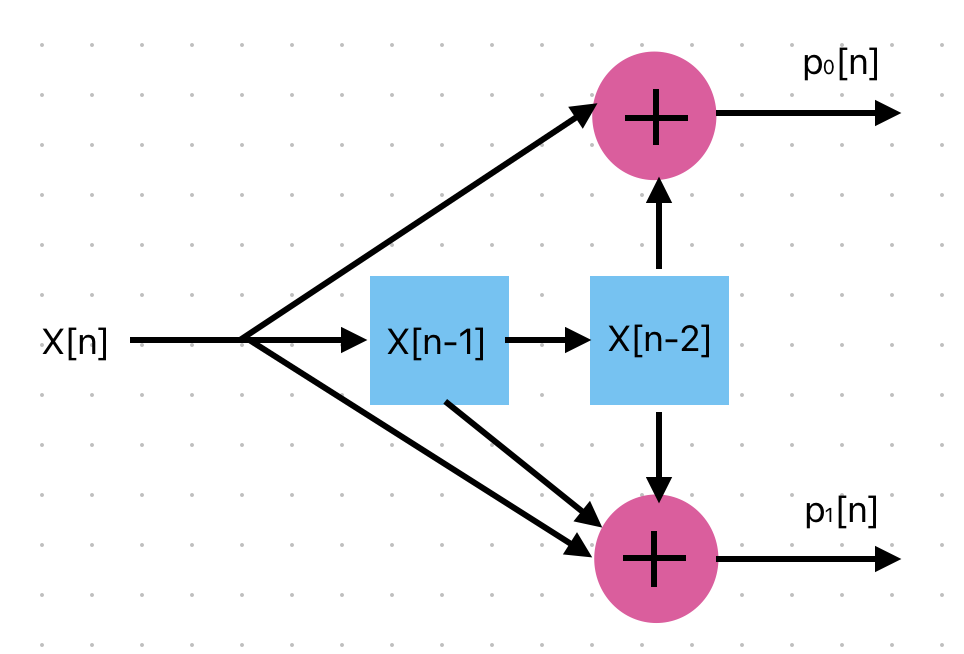
\includegraphics[width=0.6\textwidth]{Figs/Conv_Register.png}
    \caption{Caption}
    \label{fig:Conv_Register}
\end{figure}
Here \(x[n-1]\) and \(x[n-2]\) are held in two registers.  A new bit, \(x[n]\), arrives
at the left.  The box computes the parity bits from the incoming bit
\(x[n]\) and the \(2\) previous message bits.  At the end of the iteration,
the saved message bits are shifted right by one, and the incoming bit
moves into the left position.

A simpler way to represent the shift register view is to directly use the register elements, denoted by \(D\). 

\begin{figure}[h]
    \centering
    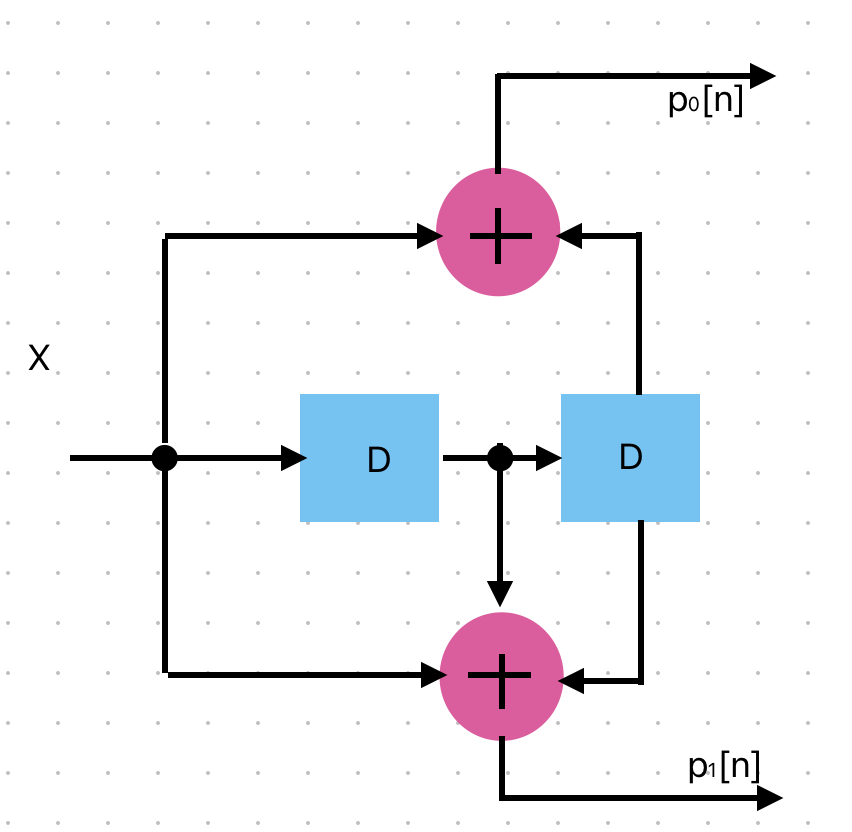
\includegraphics[width=0.6\textwidth]{Figs/Conv_FIR.png}
    \caption{Caption}
    \label{fig:Conv_Register}
\end{figure}


At the start of encoding, we assume \(x[-1]\) and \(x[-2]\) contain zero. When we finish, we add \(K-1\) zeroes to the end of the code, to allow the
registers to "settle", again at zero. For long block length, these resetting bits do not materially affect the code rate. 

\subsection{Generator Polynomial or Transfer Function}

Just like block codes, where a generator matrix is useful to describe a code, we also have generator nottaion to succinctly represent convolutional codes. In fact, we have a set of generators, where generator \(g_i\) is the generator for parity bit \(p_i\).

The generator basically shows which register contributes to the parity bit. For example, for parity stream \(p_0 = x[n] + x[n-1] + x[n-2]\), the generator polynomial \(g_0(D) = 1 + D + D^2\), or more simply \(g_0 = [111]\). For parity stream \(p_1 = x[n] + x[n-2]\), the generator is polynomial is \(g_1(D) = 1+ D^2\), or \([101]\). 

\paragraph{Transfer Function}
If we apply a z-transform to the equation \(p_0 = x[n] + x[n-1] + x[n-2]\), we have 
\[P = X(1+ D + D^2),\] so 
\[G(D) = \frac{P}{X} = 1 + D + D^2.\] 
This is know as the transfer function for the first parity bit of the convolutional code.  

The generator polynomial  relates directly to our shift-register view, as shown in  the diagram. 


With these generators, we can express the parity bits in a different way.  A convolutional code generates sequences of parity bits from
sequences of message bits by a convolution operation:

   \[p_i[n] = \sum_{j=0}^{K-1} g_i[j] x[n-j] = g \circledast x\]
where \(g_i[j]\) is the coefficient of term $D^j$,  
$K$ is, again, the constraint length. Again, \(g_i(D)\) is the K-element generator polynomial for parity bit \(p_i\).

The convolutional nature of parity bits generation leads to the name convolutional code. 

Regarding the constraint length K, the larger K is,
the more times a particular message bit is used when calculating parity bits.  This will lead to greater redundancy, and usually to better error correcting possibilities.



\section{State Space View}
In this section we briefly review the state-space approach to convolutional codes.

An \((n, k, m)\) convolutional encoder is a linear sequential device which maps a sequence of $k$-dimensional information, of input blocks \(x_1, x_2, \cdots\), over the finite field \(GF(2)\),  into a sequence of $n$-dimensional output, of output blocks \(p_1, p_2, \cdots\)

The encoder also passes through a sequence of internal $m$-dimensional state vectors, or simply states \(s_0 , s_1, \cdots\). The $j$th code block \(c_j\) is a linear function of the $j$th input block \(x_j\) and also of the $j$th state \(s_j\). This is precisely a linear system, defined over the finite field \(GF(2)\).


The formal description of the encoder’s operation is  this: the initial state \(s_0\) is assumed to be the zero state and for \(j \geq 0\), the linear system evolves as:
\begin{align}
 s_{j+1} &= s_j A + x_j B  \label{eq:state} \\
 p_j &= s_j C + x_j D \label{eq:output}
\end{align}
where the four matrices \(A, B, C,\) and \(D\) have entries from GF(2) and dimensions \(A:m \times m; B:k \times m; C:m \times n; D : k \times n\).

For the code defined in the example,  the linear system is:  
\begin{align*}
s_{j+1} &= s_j \begin{bmatrix}
    1 & 0 \\
    0 & 0
\end{bmatrix} + x_j  \begin{bmatrix}
    0 & 1 \\
\end{bmatrix} \\
p_{j} &= s_j \begin{bmatrix}
    1 & 1 \\
    1 & 0
\end{bmatrix} + x_j  \begin{bmatrix}
    1 & 1 \\
\end{bmatrix} 
\end{align*}

The \((n,k,m)\) convolutional code associated with such an encoder is then defined to be the set of all possible output sequences (or codewords) \(p_0, p_1, p_2, \cdots\) which can be produced form the encoder, starting with the initial state \(s_0 = 0\).

Let us represent the example convolutional code using the state space view. 

\begin{center}
\begin{tabular}{|c|c|c|c|}
\hline
\(x_n\) & \(s_n[0]s_n[1]\) & \(p_n[0]\) & \(p_n[1]\) \\ \hline
1 & 10 & 1 & 1 \\ 
1 & 11 & 0 & 1\\
0 & 01 & 0 & 1\\
1 & 10 & 0 & 0\\ 
0 & 01 & 1 & 0\\
0 & 00 & 1 & 0\\
\hline
\end{tabular}
\end{center}

The state transition can be represented by a state machine graph, where transitions are shown by arrows pointing from the current state to the next state. On each transition, we associate the bits \(x/p_0p_1\) where \(x\) is the input bit and \(p_0p_1\) are the two parity bits.  

\begin{figure}[h]
    \centering
    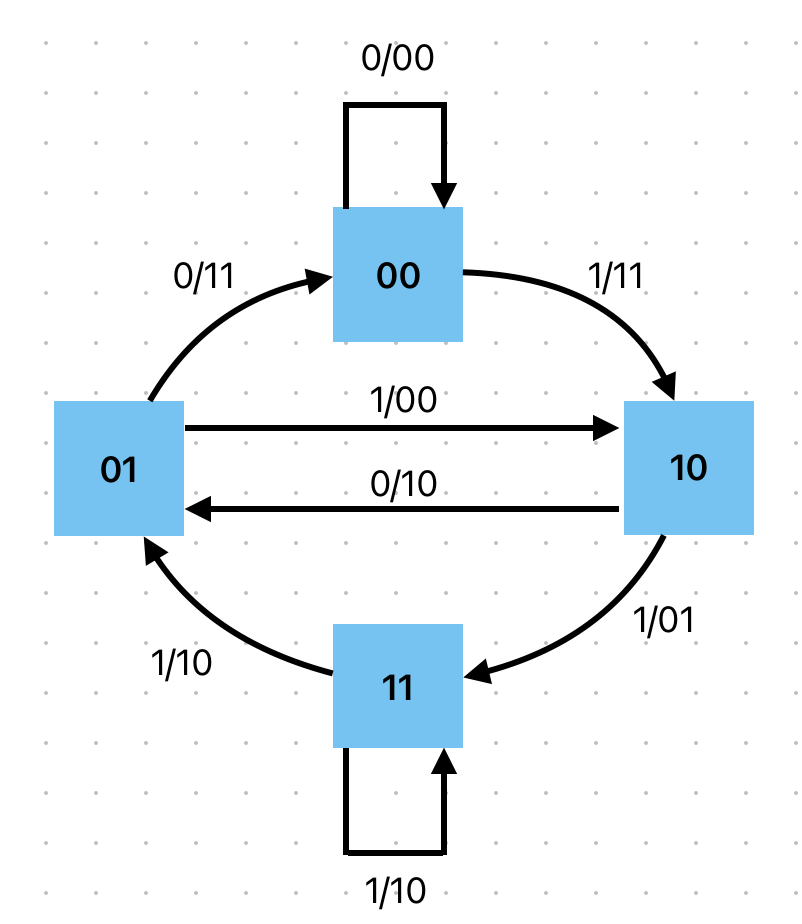
\includegraphics[width=0.6\textwidth]{Figs/ConvStateSpace.png}
    \caption{State Machine View of the Example Convolutional Codes}\label{fig:ConvStateSpace}
\end{figure}

\paragraph{Break here}

\section{Trellis View}
The state machine alone is pretty useful.  But it only gives a visual
representation of where we are at iteration n.  It would be nice to
have a representation that kept track of what states we had been in
previously.

(In fact, when we learn how to decode convolutional codes, it's going
to be \textbf{very} nice)

What we will do is, essentially, take the state machine and spread (unroll) it out over time.  This is called the "trellis" view.  With this view, we can trace a path over time; each path corresponds to a valid codeword. 

In the trellis view, we will only label the transitions with the
parity bits, instead of always including \(x[n]\).  We do this because of
the two arrows exiting a transition, the upper arrow always
corresponds to \(x[n]=1\), and the lower arrow always corresponds to
\(x[n]=0\).

Figure~\ref{fig:ConvTrellis} shows the trellis structure for our example convolutional codes. 
\begin{figure}[h]
    \centering
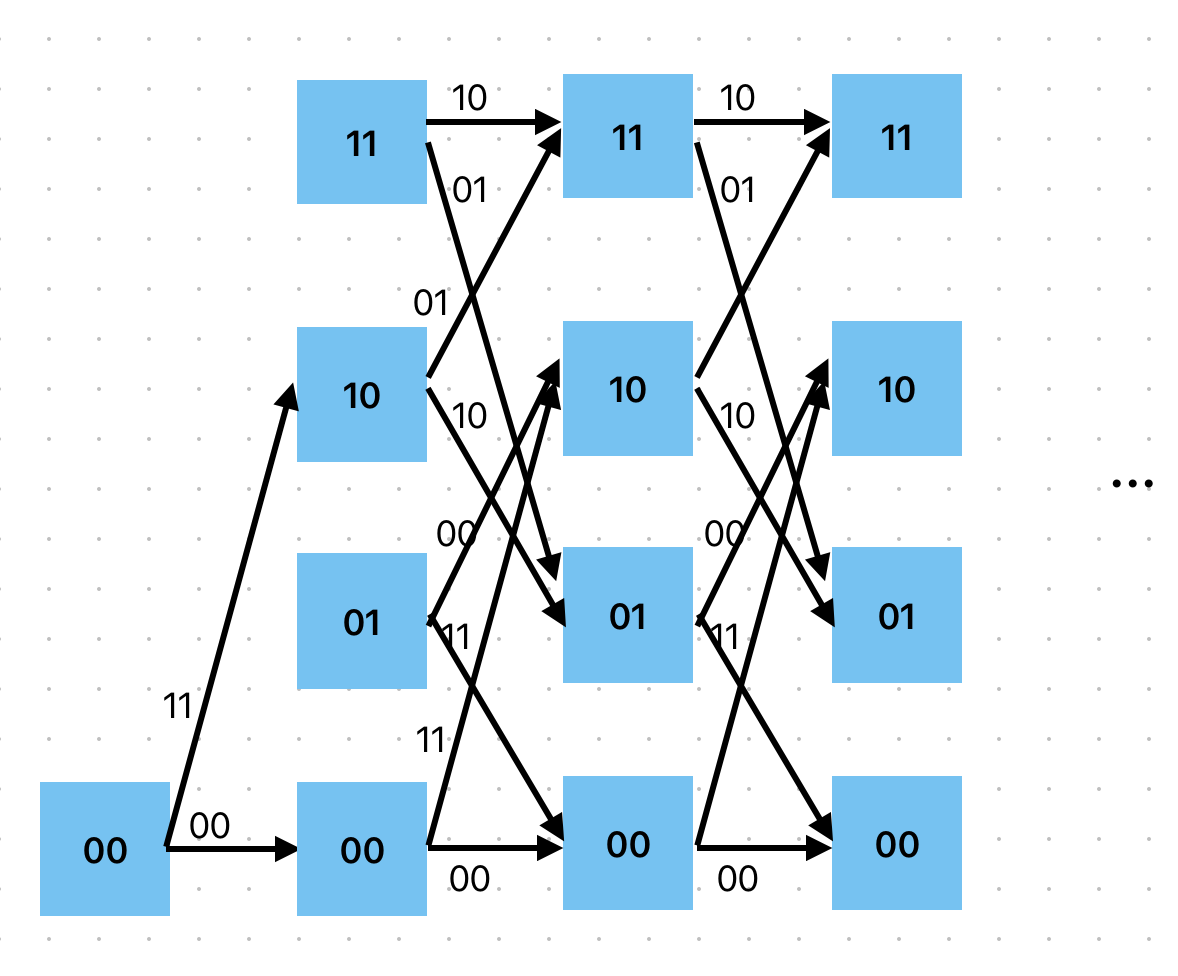
\includegraphics[width=0.6\textwidth]{Figs/ConvTrellis.png}
    \caption{State Machine View of the Example Convolutional Codes}\label{fig:ConvTrellis}
\end{figure}


Our encoding procedure now can be described straightforward:  Beginning at the starting state,
for each message bit, make the appropriate state transition, and send \(p_0p_1\).  Then end the message with \(K-1\) zeros, to ensure return to the
starting state.

Any path through the trellis corresponds to a code word.  We could
also consider the subset of paths that start in the zero state and end
at time step \(N\) in the zero state these would generate codewords of
length N. The original message bits can be read off by noting
whether the path at each stage takes the upper branch (bit \(0\)) or lower
branch (bit \(1\)). And the codeword bits can be read off from the labels
on the traversed path.

Let us show how we encode the example message bits \(
101011\). This should be a path along the states from six steps. In reality, we might need to terminate the message bits using \(00\) so that the state returns to the all zero state. 

This termination loses a bit information bit, but is not important. 

Because the states are binary strings, we can  interpret them as decimal numbers, 
  "00, 01, 10, 11" as \(0,1, 2, 3\). Such representation is useful in implementation.

\section{Free Distance of Convolution Codes}

The parity stream forms a linear code (the parity bits are linear functions of the data bits).

The fact that parity bits are linear functions of the data bits is essentially saying that \(c=Gx\), which establishes the linearity of the code.

 In view of the convolution expression for the parity bits, it follows that the sum of two
  parity streams is a parity stream (the stream corresponding to the sum of the two data words).

The smallest-weight nonzero codeword has a weight that, locally in time, plays a role analogous to \(d\) (the minimum Hamming distance). It's called the free distance of the convolutional code; we'll denote
it \(d_{free}\).

Specifically, the free distance \(d_{free}\) of a convolutional code is the minimal Hamming weight difference between the all-zeroes output and an output generated from a path starting at  all zero state and ending at all zero state. The correcting capability \(t\) of a convolutional code is the number of errors that can be corrected by the code. It can be calculated as
\(\lfloor (d-1)/2 \rfloor \). 

The \(d_{free}\) plays a similar role as minimum distance of a block code, but with a small modification. Since a convolutional code doesn't use blocks, processing instead a continuous bitstream, the value of \(t\) applies to a quantity of errors located relatively near to each other. That is, multiple groups of \(t\) errors can usually be fixed when they are relatively far apart. Free distance can be interpreted as the minimal length of an erroneous "burst" at the output of a convolutional decoder. The fact that errors appear as "bursts" should be accounted for when designing a concatenated code with an inner convolutional code. The popular solution for this problem is to interleave data before convolutional encoding, so that the outer block (usually Reed–Solomon) code can correct most of the errors.

With linear block codes, minimum distance \(d\) told us that we could correct all patterns
of up to \(\lfloor (d-1)/2 \rfloor\)  errors in a block.  In convolutional codes, \(d_{free}\) tells us something similar: we can correct \(\lfloor (d_{free} -1)/2 \rfloor \) bursty errors.


\section{Recursive Systematic Convolutional Code}
So far the convolutional code we have introduced has a forward only path. This corresponds to Finite Response Filter. It is possible, and has great advantage to include backward path in generating the parity bits. That corresponds to Infinite Response Filter. In fact, in modern coding schemes like Turbo codes, only recursive systematic convolutional codes are used. 


The recursive systematic convolutional (RSC) encoder is obtained from the nonrecursive nonsystematic (conventional) convolutional encoder by feeding back one of its encoded outputs to its input. Figure~\ref{fig:Conv_Register} shows a conventional convolutional encoder.

The RSC encoder of this conventional convolutional encoder is represented 
as \(G=[1, g / g ]\) where the first output (represented by g ) is fed back to the input.  Figure \ref{fig:Conv_RSC} shows the resulting 
RSC encoder.

\begin{figure}[h]
    \centering
    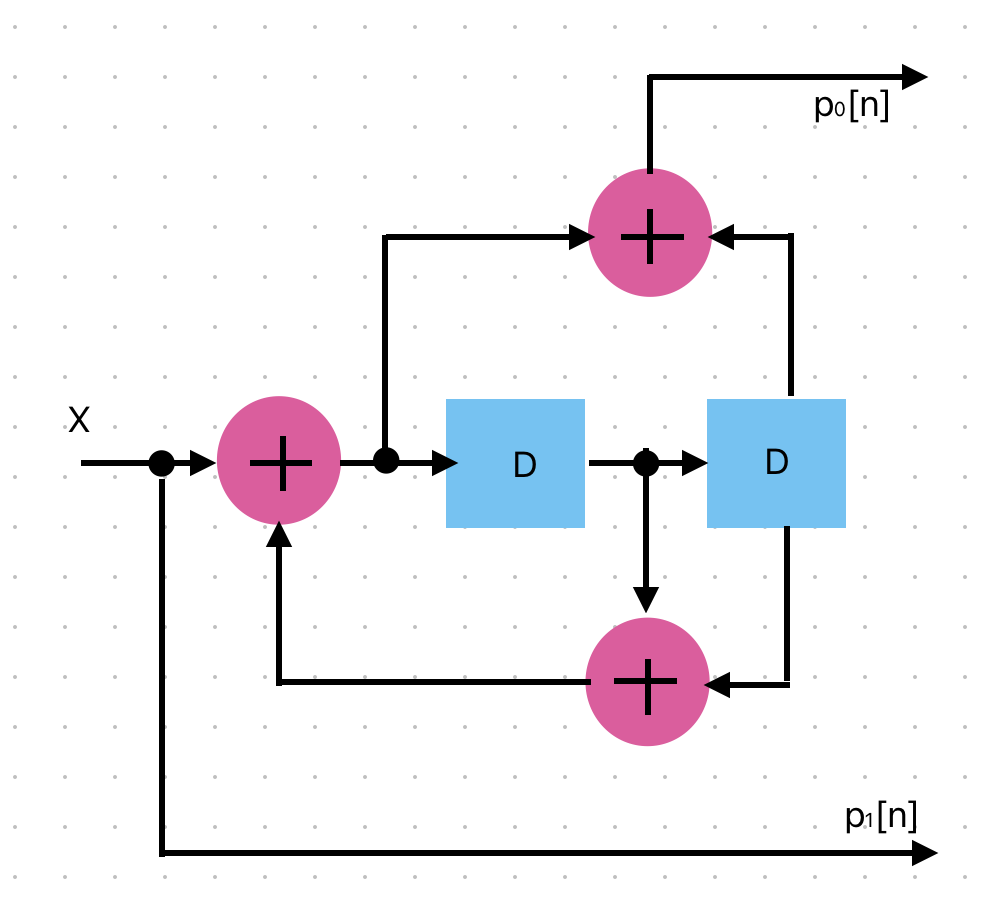
\includegraphics[width=0.6\textwidth]{Figs/Conv_RSC.png}
    \caption{Caption}
    \label{fig:Conv_RSC}
\end{figure}

The following is an extremely simple recursive systematic convolutional code. 

\begin{example}
    \textbf{Accumulator.} Figure~\ref{fig:accumulator} shows a rate \(1/2\) recursive systematic convolutional code. Assuming the input bits are \(x_1, x_2, x_3, \cdots, \), and output parity bits are \(y_1, y_2, y_3, \cdots\), then we have 
    \begin{align*}
        y_1 &= x_1 \\
        y_2 &= x_1 + x_2 \\
        y_3 &= x_1 + x_2 + x_3 \\
        \vdots \\
        y_n & = \sum_{i=1}^{n} x_i
    \end{align*}
    Such a convolutional code is called as an accumulator. In modulation, it is also commonly used as a pre-coder. The transfer function is \(\frac{1}{1+D}.\)
    
\begin{figure}[h]
    \centering
    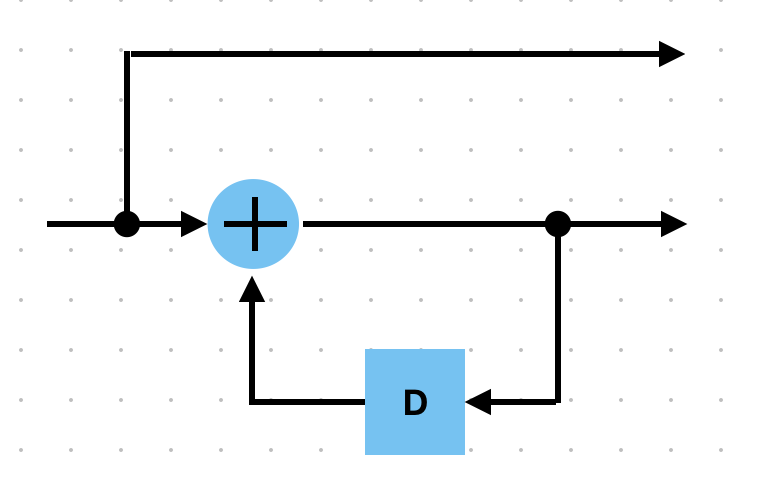
\includegraphics[width=0.6\textwidth]{Figs/Accumulator.png}
    \caption{An accumulator}
    \label{fig:accumulator}
\end{figure}

\end{example}


\subsection{Transfer Function of RSC}
The transfer function of the code defined in Fig~\ref{fig:Conv_RSC}.
We will introduce the variable \(s[n]\) to represent the value right before first register. Then we have the following equations: 
\begin{align*}
s[n] &= x[n] + s[n-1] + s[n-2] \nonumber\\
p[n] &= s[n] + s[n-2]
\end{align*}
Applying the \(z\)-transform to the two equations, we have 
\begin{align*}
S(1+D + D^2) &= X, \\
P &= S(1 + D^2).
\end{align*}
Canceling \(S\) in the above two equations gives us the transfer function: 

\begin{align}
\frac{P}{X} = \frac{1+D^2}{1+ D + D^2} \label{eq:RSCTransfer}
\end{align}

Compared with a non-recursive convolutional code, the transfer function of a recursive convolutional code has a non constant denomintor function. This provides the feedback loop.



